\documentclass[11pt]{article}

\usepackage{../../BaseStyle}

%%%%%% tables %%%%%%%%

\usepackage{array}
\renewcommand{\arraystretch}{1.5}
\setlength{\tabcolsep}{8pt}

%%%%%% plotting %%%%%%

\usepackage[dvipsnames]{xcolor}
\usepackage{tikz}
\usepackage{pgfplots}

\pgfplotsset{every axis/.append style={
        axis x line=middle,    % put the x axis in the middle
        axis y line=middle,    % put the y axis in the middle
        axis line style={<->,color=black}, % arrows on the axis
        xlabel={$x$},          % default put x on x-axis
        ylabel={$y$},          % default put y on y-axis
}}

\pgfplotsset{compat=1.14} % sometimes, everything falls apart without this

 %\usepgfplotslibrary{fillbetween} %for shading between curves

%%%%%% commands %%%%%%

\def\todo{\textcolor{red}{TODO}}

% exam heading; course name is first argument, exam information is second argument
\newcommand{\Heading}[2]{
    \fbox{
        {\Large\textbf{#1}}
    }
    \hfill
    \fbox{
        \begin{minipage}{0.2\textwidth}
            \begin{center}
                \textbf{#2}
            \end{center}
        \end{minipage}
    }
\par\vspace{0.1in}}

% for being lazy while beautifying integrals
\newcommand{\dint}{\displaystyle\int}

% for being lazy while beautifying limits
\newcommand{\dlim}{\displaystyle\lim}

%%%%%% stuff %%%%%%

\usepackage{fancyhdr}

%\setcounter{page}{0} % first page is page 0

\parindent0pt % no indent

\fboxsep=0.25cm % little space in fbox border

%%%%%% BEGIN! %%%%%%%
\begin{document}


\Heading{MATH 1210}{Review for Final}

\vspace{0.1in}

\textbf{Name} \hrulefill
\smallskip{}

\begin{itemize}
    \item[\textbf{D1.}] A device measuring ocean temperature is placed into the ocean at time $t=0$ minutes and begins recording the temperature $T$ (in ${}^{\circ}$ C) of the ocean water as it descends.

        \begin{enumerate}
            \item In terms of the context above, what does $T'(20)$ represent? What are its units of measurement? You may simply write your answers with no justification.
                \vfill
            \item In terms of the context above, what does $\displaystyle\frac{T(30)-T(20)}{30-20}$ represent? What are its units of measurement? You may simply write your answers with no justification.
                \vfill
            \item  The graph below depicts the temperature measurements of the device at different times.

    %temperature at the surface is 20 degrees C
    %held for 5 minutes then sinks at a rate of 100 meters per minute
    %after 5 minutes, its depth is still 0 and temperature is still 20
    %after 6 minutes, its depth is 100 meters
    %after 15 minutes, its depth is 1000 meters and temperature is 22-10*1=4
    %after 65 minutes, its depth is 5000 meters and temperature is 10-0.1*50=5

                \begin{center}
                    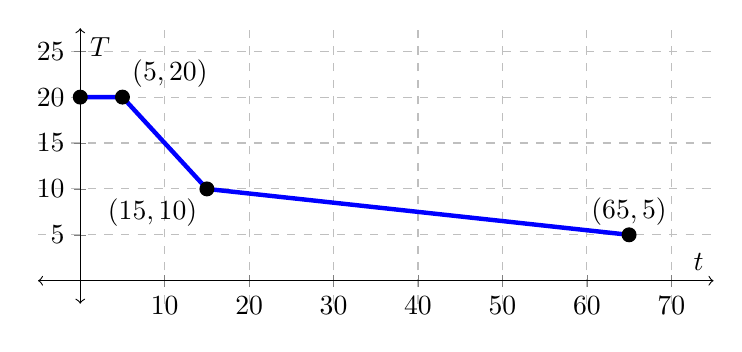
\begin{tikzpicture}
                        \begin{axis}[
            %    axis y line = left,
            %    axis x line = bottom,
                            xlabel = {$t$},
                            ylabel = {$T$},
                            ytick       = {5,10,15,20,25},
                            yticklabels = {$5$,$10$,$15$,$20$,$25$},
                            xtick       = {10,20,30,40,50,60,70},
                            xticklabels = {$10$,$20$,$30$,$40$,$50$,$60$,$70$},
                            samples     = 320,
                %domain      = 0:4,
                %restrict y to domain=-5:5,
                            ymin = -2.5, ymax = 27.5,
                            xmin = -5, xmax = 75,
                            width=4in,height=2in,
                            grid=both, grid style=dashed
                            ]
             %
                            \draw[ultra thick,blue] (0,20) -- (5,20) -- (15,10) -- (65,5);
                            \filldraw (0,20) circle (2.5pt);
                            \filldraw (5,20) circle (2.5pt) node[anchor=south west]{$(5,20)$};
                            \filldraw (15,10) circle (2.5pt) node[anchor=north east]{$(15,10)$};
                            \filldraw (65,5) circle (2.5pt) node[anchor=south]{$(65,5)$};
             %\addplot[blue, ultra thick, mark=none, smooth] {4-x^2};
             %
             %\addplot[blue, ultra thick, mark=none, smooth] coordinates{ (0,.61) (0.25,2.92) (0.5,0.8) (0.75,1) (1,.77) (1.25,1.34) (1.5,.74) (1.75,1.25) (2,1.47) (2.25,2.46) (2.5,3.23) (2.75,3.71) (3,5.29) (3.25,3.38) (3.5,1.11) (3.75,2.29)};
             %
                        \end{axis}
                    \end{tikzpicture}    
                \end{center}
                For each answer choice below, circle the answer choice if and only if the statement for that answer choice is TRUE.\\

                \begin{minipage}[t][1.5in]{0.2\textwidth}
                    \begin{itemize}
                        \item[A.] $\dfrac{dT}{dt}\bigg|_{t=3}=0$
                            \vfill

                        \item[B.] $\dfrac{dT}{dt}\bigg|_{t=3}<0$
                            \vfill

                        \item[C.] $\dfrac{dT}{dt}\bigg|_{t=3}>0$
                            \vfill

                    \end{itemize}
                \end{minipage}
                \hfill
                \begin{minipage}[t][1.5in]{0.2\textwidth}
                    \begin{itemize}
                        \item[D.] $T'(10)<0$
                            \vfill

                        \item[E.] $T'(10)>0$
                            \vfill

                        \item[F.] $T'(10)=0$
                            \vfill

                    \end{itemize}
                \end{minipage}        

        \end{enumerate}
        \pagebreak
    \item[\textbf{D2.}] Write down the derivatives of the following functions. No work required. No need to simplify.

        If you need to write down your work, please do so at the bottom half of this page, not in the answer space.

        \begin{center}
            \begin{tabular}{l c r l c r}
            %
                $\displaystyle\frac{d}{dx}\left[ -4x^{9} \right]$ & $=$ & \rule[-8pt]{1.5in}{0.4pt} &
                \vspace{4cm}
            %
                $\displaystyle\frac{d}{dx}\left[ \dfrac{2}{\sqrt{x^3}} \right]$ & $=$ & \rule[-8pt]{1.5in}{0.4pt}\\[0.3in]
                \vspace{4cm}
            %%%%%
                $\displaystyle\frac{d}{dx}\left[ 4^x \right]$ & $=$ & \rule[-8pt]{1.5in}{0.4pt} & 
            %%%%%
                $\displaystyle\frac{d}{dx}\left[ \frac{\pi^2}{6} \right]$ & $=$ & \rule[-8pt]{1.5in}{0.4pt}\\[0.3in]
                \vspace{4cm}
            %%%%%
                $\displaystyle\frac{d}{dx}\left[ x^2 + x+1 \right]$ & $=$ & \rule[-8pt]{1.5in}{0.4pt}&
            %
                $\displaystyle\frac{d}{dx}\left[ \ln(x) + x \right]$ & $=$ & \rule[-8pt]{1.5in}{0.4pt}\\[0.3in]
                \vspace{3cm}
            %%%%%
                $\displaystyle\frac{d}{dx}\left[ \log_2(x^5) \right]$ & $=$ & \rule[-8pt]{1.5in}{0.4pt} & 
            %
                $\displaystyle\frac{d}{dx}\left[ \frac{1}{x} + \frac{2}{x^2} \right]$ & $=$ & \rule[-8pt]{1.5in}{0.4pt}\\[0.3in]
            %%%%%
            \end{tabular}

        \end{center}        \pagebreak

    \item[\textbf{D3.}]Find the following derivative:

        \[ \dfrac{d}{dx} \left[ \left( \dfrac{x^3-6x^2}{2x+1} \right) \cdot \ln(3^{x+1}) \right]\]
        \pagebreak

    \item[\textbf{I1.}] You may simply record your answers with no work shown. Please show your work to part (b). ({\bf Note:} Below, ``NOTOA" means ``none of the other answers".)
        \begin{itemize}

            \item[(a)] Suppose $f$ is a continuous function of the variable $t$, $0\leq t\leq 24$. If $f$ is measured in megawatts (MW) and $t$ is measured in hours (hr), then what are the units of $\displaystyle\int_0^{24} f(t)\,dt$?\\

                \,\hfill
                \fbox{A} MW/hr$^2$
                \hfill
                \fbox{B} MW/hr
                \hfill
                \fbox{C} MW
                \hfill
                \fbox{D} hr
                \hfill
                \fbox{E} NOTOA
                \hfill\,\\
                \medskip{}

            \item[(b)] If $p(t)$ represents the (instantaneous) rate of change of levels (in parts per million) of an airborne pollutant $t$ hours after midnight on a given day, then what does $\displaystyle\int_6^{12} p(t)\,dt$ represent in this context?
                \vspace{6cm}

            \item[(c)] Let $T'(t)$ represent the (instantaneous) rate of change (in $^{\circ}$C/hour) of temperature in Charlottesville at a time $t$ (in hours) during a particular day. Assume the temperature was highest at 5:00 PM and lowest at 4:00 AM. Which of the following integrals are {\bf positive}? Circle all correct answers.\\[0.2in]
    %
                \,\hfill
                \fbox{A} $\displaystyle\int_{12}^{17} T'(x)\,dx$
                \hfill
                \fbox{B} $\displaystyle\int_{17}^{22} T'(x)\,dx$
                \hfill
                \fbox{C} $\displaystyle\int_1^4 T'(x)\,dx$
                \hfill
                \fbox{D} $\displaystyle\int_4^{10} T'(x)\,dx$
                \hfill
                \fbox{E} NOTOA        
        \end{itemize}
        \pagebreak

    \item[\textbf{I3.}] Write down the indefinite integrals of the following expressions. 

        Although no work is required, you are encouraged to include any work that shows your thought process. 

%constant, power, exponential, log, +C, algebraic manipulation

        \begin{center}
            \begin{tabular}{l c r l c r}
            %
                $\displaystyle\int 5\,dx$ & $=$ & \rule[-8pt]{1.5in}{0.4pt} &
                \vspace{5cm}

            %
            %$\displaystyle\int \,dx$ & $=$ & \rule[-8pt]{1.5in}{0.4pt}\\[0.3in]
            %%%%%
            %$\displaystyle\int 15\,dx$ & $=$ & \rule[-8pt]{1.5in}{0.4pt} & 
            %%%%%
            $\displaystyle\int \dfrac{1}{x^6} \,dx$ & $=$ & \rule[-8pt]{1.5in}{0.4pt}\\[1in]
            \vspace{5cm}

            %%%%%
            $\displaystyle\int 2^x\,dx$ & $=$ & \rule[-8pt]{1.5in}{0.4pt}&
            %
            $\displaystyle\int x^2 + 3x^4\,dx$ & $=$ & \rule[-8pt]{1.5in}{0.4pt}\\[1in]
            %%%%%
            $\displaystyle\int x^{-1} \,dx$ & $=$ & \rule[-8pt]{1.5in}{0.4pt} & 
            %
            $\displaystyle\int e^5 \,dx$ & $=$ & \rule[-8pt]{1.5in}{0.4pt}\\[0.3in]
            %%%%%
        \end{tabular}
    \end{center}        \pagebreak

\item[\textbf{I4.}] 
    \begin{enumerate}[label=(\alph*)]

        \item On which of the following integrals could the Fundamental Theorem of Calculus NOT be used? Circle \textbf{all} the correct answers, and then evaluate the remaining ones.

            \,\hfill
            \fbox{A} $\displaystyle\int_{-1}^1 \ln (x^2)\dd{x}$
            \hfill
            \fbox{B} $\displaystyle\int_{-1}^3 \frac1{x^2-4}\dd{x}$
            \hfill
            \fbox{C} $\displaystyle\int_{2}^{-4} 2^x\dd{x}$
            \hfill
            \fbox{D} $\displaystyle\int_{-2}^{0} e^{\sqrt{x}} \dd{x}$
            \hfill\

            \vspace{5cm}

        \item Evaluate the integral:
            \[
                \int_{1}^3 \frac{x+2x^2}{x^2} \dd{x}
            \]
    \end{enumerate}
    \pagebreak

\item[\textbf{L2.}] For each limit below, first determine the form of the limit, then find the value of the limit. 
    If the given function is continuous at the target, you may simply write ``n/a'' for the form. 
    Show complete work --- using mathematics and/or words --- to justify your answers. 
    ({\it Note:} $e \approx 2.718$.)


    \begin{enumerate}
        \item[(a)] $\displaystyle\lim_{x\to\infty} \frac{e^{5x}+ \ln(x)}{x^{5} - 2}$
            \hspace{1cm}
            \textbf{form:} \rule[-6pt]{1.25in}{0.4pt} \quad
            \textbf{value:} \rule[-6pt]{1.25in}{0.4pt}
            \vspace{5cm}

        \item[(b)] 
            $\displaystyle\lim_{x\to0} \frac{\ln(1+x)-e^{2x}}{x-1}$
            \hspace{1cm}
            \textbf{form:} \rule[-6pt]{1.25in}{0.4pt} \quad
            \textbf{value:} \rule[-6pt]{1.25in}{0.4pt}
            \vspace{5cm}

        \item[(c)] 
            $\displaystyle\lim_{x\to 0^{+}} \frac{\sqrt{1+x}}{\ln(x)}$
            \hspace{1cm}
            \textbf{form:} \rule[-6pt]{1.25in}{0.4pt} \quad
            \textbf{value:} \rule[-6pt]{1.25in}{0.4pt}
            \vspace{0.3in}
    \end{enumerate}        \pagebreak

\item[\textbf{A3.}] A particular type of window is composed of a semicircle placed atop a rectangle. If 20 feet of framing material are available for the outer frame of the window, then what radius $r$ of the semicircle maximizes the area of the entire window?\\

    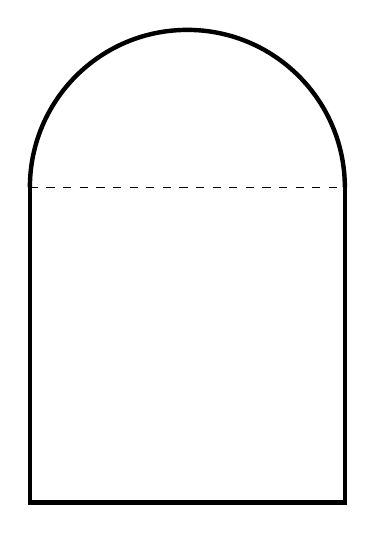
\begin{tikzpicture}
        \draw[ultra thick] (-2,2) arc (180:0:2);
        \draw[ultra thick] (-2,2) -- (-2,-2) -- (2,-2) -- (2,2);
        \draw[dashed] (-2,2) -- (2,2);
    \end{tikzpicture}        \pagebreak

\item[\textbf{P1.}] Suppose you roll two 4-sided dice, and then compute the difference of the second roll from the first. Let \( X \) be the random variable taking this difference as its value.
    \begin{enumerate}[label=(\alph*)]

        \item Is \( X \) continuous or discrete? What is its support?
            \vspace{3cm}

        \item What is the sample space for the experiment?
            \vspace{3cm}

        \item Find the probability mass function of \( X \).
            \vspace{5cm}

        \item Find the expectation of \( X \).

    \end{enumerate}

    \pagebreak

\item[\textbf{P2.}] The expected value (or mean) of a continuous random variable $X$ is $\displaystyle \mu=E[X]=\int_1^5k \dd{x}$ where $k$ is an unknown constant that we will find later. 
    \begin{enumerate}[label=(\alph*)]

        \item What is the probability density function $p(x)$? Your answer will involve $k$.
            \vspace{3cm}

        \item Find the value of $k$ to ensure that $p(x)$ is a pdf. What is the support of \( X \)?
            \vspace{3cm}

        \item Find the cumulative distribution function (CDF) $C(x)$.
            \vspace{3cm}

        \item Use $C(x)$ to find $P(X \leq 4)$.
            \vspace{3cm}

        \item Find the expectation and variance (without \( k \)) of \( X \).

    \end{enumerate}
\end{itemize}
\end{document}
